\section{Results}

\subsection{Uniaxial and EB strain analysis} \label{c2:sec:uniaxialandEBresults}

    It was observed under these tests that the resulting stress–strain responses transitioned to a linear region prior to failure (Fig. \ref{c2:fig:3}). This observation supported the use of a collagen fiber recruitment model for MV tissue (Section \ref{sec:generalconsiderations}). Under EB strain testing kinematics, full recruitment was reached on average at a mean and standard deviation value of $0.284\pm0.047$ in Green’s strain and $782.1\pm121.5$ kPa in ensemble stress for the anterior leaflet. For the posterior leaflet, full recruitment strain was achieved at $0.2730\pm0.0156$ in Green strain and $1434.0\pm165.4$ kPa in ensemble stress. The posterior leaflet appeared to recruit more gradually than that of the anterior leaflet, with an average $\sigma_r$ (the standard deviation of the collagen fiber recruitment function) of $0.0231\pm0.001$ in Green strain compared to $0.015\pm0.003$ for the anterior leaflet. In comparison, the average maximum tensile strength under uniaxial loading along the circumferential direction for the anterior leaflet was 2, $220.1\pm794.5$ kPa. This suggests that the stress required to tear the tissue is approximately three times higher than the stress required to reach full recruitment on average.
    

\subsection{Parameter estimation}

    For the fitted parameters obtained from uniaxial extension and EB strain datasets (Section \ref{c2:sec:2254}, Table \ref{c2:tab:4}, Table \ref{c2:tab:5}), we observed similar collagen modulus $\eta_c$ for both tests. There appeared to be a shift in strain for the recruitment parameters values due to the differences in testing methodology. For all specimens tested under the full planar tension test protocols, they demonstrated a clear toe region at stresses below 7 kPa. This gave us a good initial estimate of the elastin response in comparison to the final fitted values, while fitting the high stress region resulted in recruitment parameter values that were consistent with EB strain testing (Fig. \ref{c2:fig:4}a). The fit of the full model (Eqn. \ref{eqn:multilayeredstressform}) (Fig. \ref{c2:fig:4}b) had a very good mean R-squared value of 0.964 for the anterior leaflet and 0.951 for the posterior leaflet (Table \ref{c2:tab:6}, Table \ref{c2:tab:7}). The full model (Eqn. \ref{eqn:multilayeredstressform}) was used to predict the stress of the extra-physiological protocols and obtained similar results (Fig. \ref{c2:fig:4}c and d). The modulus of the collagen fibers was found to be $164.0 \pm 16.4$ MPa for the anterior and posterior leaflets under planar tension, which is comparable for all mechanical data (Fig. \ref{c2:fig:5}a, Table \ref{c2:tab:4}, \ref{c2:tab:5}, \ref{c2:tab:6}, \ref{c2:tab:7}).
    
    
\begin{table}
\centering
\caption{Uniaxial extension testing results for the MV anterior leaflet.}\label{c2:tab:4}
\begin{tabular}{L{.5in}L{0.8in}L{0.6in}L{0.6in}L{0.6in}}
\hline
 & $\mathbf{\eta}_c \mathrm{(MPa)}$  & $\mu_r^f$ & $\sigma_r^f$ & $E_{ub}^f$  \\
\hline
1 & 68.2420 & 0.12543 & 0.01602 & 0.1434    \\
2 & 345.6285 & 0.23445 & 0.02099 & 0.2558   \\
3 & 114.5181 & 0.13822 & 0.02682 & 0.1592   \\
4 & 25.7835 & 0.11667 & 0.02545 & 0.1592    \\
\hline
Mean & 138.5431 & 0.15369 & 0.02232 & 0.1794    \\
SEM & 71.3667 & 0.02728 & 0.00244 & 0.0257      \\
\hline
\end{tabular}
\end{table}


\begin{table}
\centering
\caption{Equibiaxial strain testing results.}\label{c2:tab:5}
\begin{tabular}{L{.4in}L{.5in}L{.5in}L{.5in}L{.5in}L{.5in}L{.5in}L{.5in}L{.5in}}
\hline
 & \multicolumn{4}{l}{\textbf{Anterior}} & \multicolumn{4}{l}{\textbf{Posterior}}   \\
 \hline
 & $\mathbf{\eta}_c$  & $\mu_r^f$ & $\sigma_r^f$ & $E_{ub}^f$ 
 & $\mathbf{\eta}_c$  & $\mu_r^f$ & $\sigma_r^f$ & $E_{ub}^f$        \\
 \hline
1 & 83.93 & 0.270 & 0.023 & 0.298 & 151.06 & 0.200 & 0.022 & 0.224    \\
2 & 146.67 & 0.187 & 0.009 & 0.194 & 118.51 & 0.272 & 0.023 & 0.293   \\
3 & 218.24 & 0.178 & 0.008 & 0.184 & 149.48 & 0.260 & 0.024 & 0.287   \\
4 & 143.29 & 0.280 & 0.023 & 0.302 & 155.48 & 0.222 & 0.021 & 0.250   \\
5 & 188.67 & 0.427 & 0.013 & 0.442 & 127.20 & 0.283 & 0.026 & 0.311   \\
\hline
Mean & 156.16 & 0.268 & 0.015 & 0.284 & 140.34 & 0.247 & 0.023 & 0.273      \\
SEM & 22.78 & 0.045 & 0.003 & 0.047 & 7.338 & 0.016 & 0.0008 & 0.0156       \\
\hline
\end{tabular}
\end{table}


%%%%%%%%%%%%%%%%%%%%	begin FIGURE 	%%%%%%%%%%%%%%%%%%%%
\begin{figure}
\centering
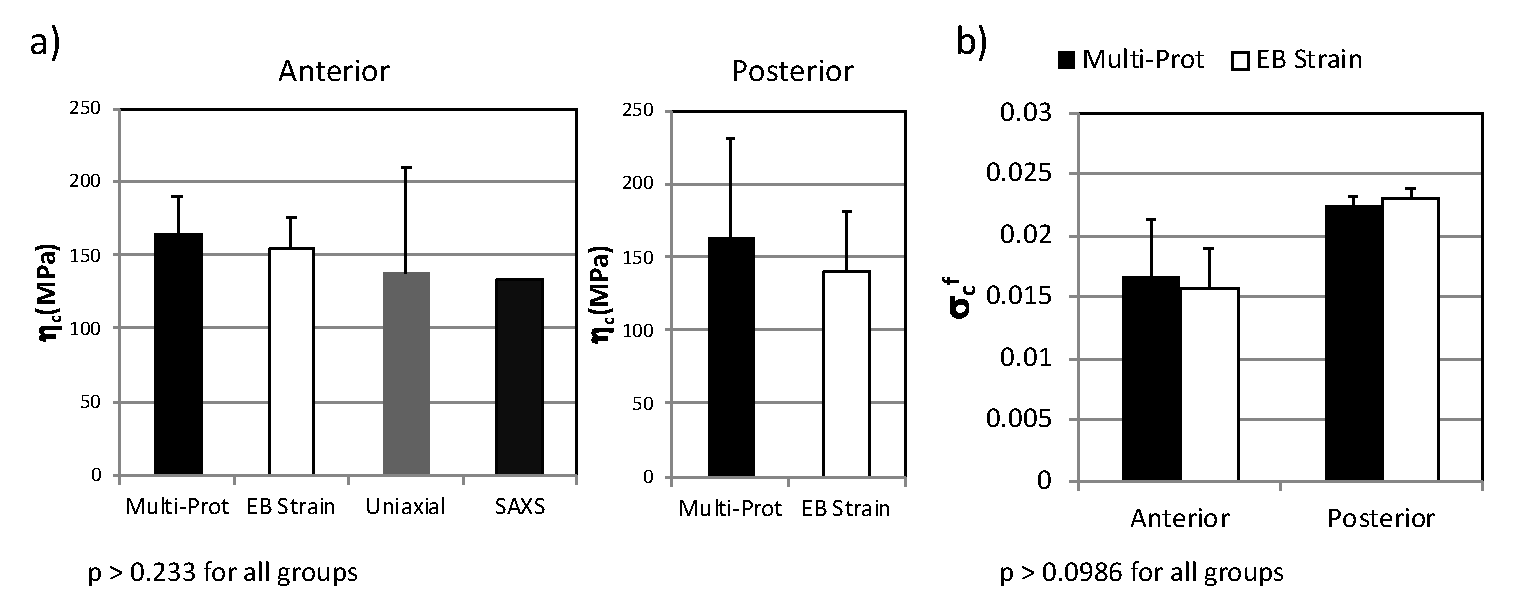
\includegraphics[width=\textwidth]{Images/chapter2/figure5.pdf}
\caption{(a) The mean and standard deviation of the collagen fiber modulus as determined from uniaxial, equibiaxial strain, and planar biaxial stress testing for both the anterior and posterior leaflets is shown. No statistical significant was found from ANOVA and student-t tests. (b) The mean and standard deviation of $\sigma_r$, which is standard deviation of the recruitment distribution of collagen fibers, in the fibrosa layer for both the anterior and posterior leaflet is shown. Again, no statistical significance was found, but the posterior leaflet appears to have larger $\sigma_r$ based on the trend.}
\label{c2:fig:5}
\end{figure}
%%%%%%%%%%%%%%%%%%%%	 end FIGURE 	%%%%%%%%%%%%%%%%%%%%


\begin{sidewaystable}
\centering
\caption{Parameter estimation results from the MV anterior leaflet.}\label{c2:tab:6}
\begin{tabular}{L{.5in}L{.55in}L{.4in}L{.4in}L{.4in}L{.4in}L{.4in}L{.4in}L{.4in}L{.4in}L{.4in}L{.4in}L{.4in}}
\hline
& \multicolumn{12}{c}{\textbf{Collagen}}    \\
\cline{2-13}
& \textbf{Modu.} & \multicolumn{4}{c}{\textbf{Fibrosa + Ventricularis}} & \multicolumn{4}{c}{\textbf{Atrialis}} & \multicolumn{3}{c}{\textbf{Spongiosa}}  \\
\hline
\textbf{ID} & $\mathbf{\eta}_c$ & $\sigma_c^f$ & $\mu_r^f$ & $\sigma_r^f$ & $E_{ub}^f$ & $\sigma_c^a$ & $\mu_r^a$ & $\sigma_r^a$ & $E_{ub}^a$ & $\mu_r^s$ & $\sigma_r^s$ & $E_{ub}^s$   \\
\hline
1 & 144.92 & 0.163 & 0.210 & 0.010 & 0.223 & 0.465 & 0.864 & 0.042 & 0.989 & 0.790 & 0.015 & 0.835  \\
2 & 86.23 & 0.140 & 0.522 & 0.010 & 0.537 & 0.077 & 1.172 & 0.019 & 1.204 & 1.177 & 0.038 & 1.256   \\
3 & 235.26 & 0.075 & 0.425 & 0.041 & 0.494 & 0.075 & 0.613 & 0.028 & 0.653 & 0.676 & 0.015 & 0.720  \\
4 & 199.33 & 0.136 & 0.293 & 0.011 & 0.307 & 0.075 & 0.914 & 0.010 & 0.927 & 0.890 & 0.010 & 0.902  \\
5 & 207.55 & 0.149 & 0.391 & 0.006 & 0.397 & 0.400 & 1.791 & 0.154 & 2.099 & 1.798 & 0.006 & 1.810  \\
6 & 196.41 & 0.180 & 0.286 & 0.015 & 0.307 & 0.250 & 0.520 & 0.019 & 0.545 & 0.525 & 0.015 & 0.559  \\
7 & 69.35 & 0.222 & 0.275 & 0.024 & 0.300 & 0.075 & 0.472 & 0.015 & 0.517 & 0.540 & 0.026 & 0.617   \\
Mean & 162.72 & 0.153 & 0.335 & 0.017 & 0.361 & 0.170 & 0.759 & 0.022 & 0.806 & 0.766 & 0.020 & 0.815   \\
SEM & 26.16 & 0.020 & 0.047 & 0.005 & 0.051 & 0.066 & 0.111 & 0.005 & 0.113 & 0.100 & 0.004 & 0.103 \\


\hline
& \multicolumn{8}{c}{\textbf{Elastin}} & & \textbf{Mat.} & \textbf{Ori.} & \textbf{$R^2$}  \\
\cline{2-13}
& \multicolumn{3}{c}{\textbf{Ventricularis}} & \multicolumn{3}{c}{\textbf{Atrialis}} & \multicolumn{2}{c}{\textbf{Spongiosa}} & & & &  \\
\hline
\textbf{ID} & $\mathbf{\eta}_e^v$ & $d^v$ & $\sigma_e^v$ & $\mathbf{\eta}_e^v$ & $d^v$ & $\sigma_e^v$ & $\mathbf{\eta}_e^v$ & $d^v$ & & $\mathbf{\eta}_m$ & $\mu_\theta$ &    \\
\hline
1 & 53.91 & 2.878 & 0.077 & 125.0 & 1.732 & 0.078 & 54.67 & 2.747 & & 0.000 & 0.304 & 0.980   \\
2 & 0.07 & 3.416 & 0.079 & 0.12 & 2.982 & 0.082 & 0.04 & 1.742 & & 0.010 & 0.350 & 0.893      \\
3 & 12.25 & 3.500 & 0.077 & 27.21 & 3.000 & 0.079 & 0.06 & 2.986 & & 0.000 & 0.622 & 0.957    \\
4 & 14.52 & 3.000 & 0.076 & 67.28 & 1.000 & 0.151 & 0.00 & 2.048 & & 0.000 & 0.384 & 0.986    \\
5 & 2.08 & 2.980 & 0.106 & 0.05 & 1.681 & 0.340 & 0.00 & 1.553 & & 0.911 & -0.05 & 0.970     \\
6 & 13.71 & 3.443 & 0.081 & 287.3 & 2.132 & 0.097 & 0.00 & 2.824 & & 0.281 & 0.449 & 0.996    \\
7 & 2.33 & 1.886 & 0.199 & 0.34 & 2.704 & 0.341 & 0.00 & 3.000 & & 0.000 & -0.20 & 0.970     \\
Mean & 16.13 & 3.021 & 0.098 & 84.55 & 2.258 & 0.138 & 9.13 & 2.558 & & 0.049 & 0.274 & 0.964 \\
SEM & 7.9 & 0.250 & 0.020 & 44.94 & 0.324 & 0.042 & 9.13 & 0.217 & & 0.047 & 0.102 & 0.015    \\
\hline
\end{tabular}
\end{sidewaystable}



\begin{sidewaystable}
\centering
\caption{Parameter estimation results from the MV Posterior leaflet.}\label{c2:tab:7}
\begin{tabular}{L{.5in}L{.55in}L{.4in}L{.4in}L{.4in}L{.4in}L{.4in}L{.4in}L{.4in}L{.4in}L{.4in}L{.4in}L{.4in}}
\hline
& \multicolumn{12}{c}{\textbf{Collagen}}    \\
\cline{2-13}
& \textbf{Modu.} & \multicolumn{4}{c}{\textbf{Fibrosa + Ventricularis}} & \multicolumn{4}{c}{\textbf{Atrialis}} & \multicolumn{3}{c}{\textbf{Spongiosa}}  \\
\hline
\textbf{ID} & $\mathbf{\eta}_c$ & $\sigma_c^f$ & $\mu_r^f$ & $\sigma_r^f$ & $E_{ub}^f$ & $\sigma_c^a$ & $\mu_r^a$ & $\sigma_r^a$ & $E_{ub}^a$ & $\mu_r^s$ & $\sigma_r^s$ & $E_{ub}^s$   \\
\hline
1 & 200.000 & 0.352 & 0.300 & 0.011 & 0.314 & 0.400 & 0.487 & 0.033 & 0.539 & 1.554 & 0.168 & 2.020 \\
2 & 197.276 & 0.247 & 0.393 & 0.010 & 0.411 & 0.400 & 0.840 & 0.051 & 0.966 & 1.911 & 0.157 & 2.218 \\
3 & 96.535 & 0.422 & 0.715 & 0.044 & 0.760 & 0.427 & 2.500 & 0.158 & 2.966 & 1.329 & 0.020 & 1.369  \\
4 & 160.354 & 0.216 & 0.543 & 0.010 & 0.558 & 0.400 & 1.323 & 0.052 & 1.436 & 2.028 & 0.018 & 2.079 \\
5 & 200.000 & 0.370 & 0.454 & 0.033 & 0.501 & 0.104 & 1.366 & 0.048 & 1.480 & 0.780 & 0.037 & 0.824 \\
6 & 181.100 & 0.292 & 0.608 & 0.017 & 0.639 & 0.400 & 1.380 & 0.079 & 1.563 & 1.079 & 0.039 & 1.196 \\
7 & 112.588 & 0.325 & 0.392 & 0.032 & 0.428 & 0.400 & 0.699 & 0.064 & 0.890 & 1.668 & 0.107 & 1.811 \\
Mean & 163.979 & 0.318 & 0.486 & 0.022 & 0.516 & 0.362 & 1.228 & 0.069 & 1.406 & 1.478 & 0.078 & 1.645  \\
SEM & 16.330 & 0.027 & 0.054 & 0.005 & 0.057 & 0.043 & 0.251 & 0.016 & 0.296 & 0.169 & 0.025 & 0.197    \\



\hline
& \multicolumn{8}{c}{\textbf{Elastin}} & & \textbf{Mat.} & \textbf{Ori.} & \textbf{$R^2$}  \\
\cline{2-13}
& \multicolumn{3}{c}{\textbf{Ventricularis}} & \multicolumn{3}{c}{\textbf{Atrialis}} & \multicolumn{2}{c}{\textbf{Spongiosa}} & & & &  \\
\hline
\textbf{ID} & $\mathbf{\eta}_e^v$ & $d^v$ & $\sigma_e^v$ & $\mathbf{\eta}_e^v$ & $d^v$ & $\sigma_e^v$ & $\mathbf{\eta}_e^v$ & $d^v$ & & $\mathbf{\eta}_m$ & $\mu_\theta$ &    \\
\hline
1 & 83.48 & 2.866 & 0.129 & 789.7 & 1.686 & 0.400 & 234.7 & 2.610 & & 0.001 & -0.60 & 0.993  \\
2 & 1.537 & 2.705 & 0.082 & 0.029 & 3.000 & 0.085 & 0.011 & 1.000 & & 0.000 & -0.04 & 0.967  \\
3 & 0.743 & 2.918 & 0.349 & 0.000 & 2.999 & 0.400 & 0.000 & 2.549 & & 0.000 & -0.31 & 0.864  \\
4 & 0.685 & 2.884 & 0.078 & 1.223 & 1.006 & 0.092 & 0.041 & 2.874 & & 0.000 & 1.425 & 0.930   \\
5 & 0.198 & 1.044 & 0.285 & 2.993 & 2.116 & 0.393 & 0.778 & 3.000 & & 0.426 & -0.39 & 0.972  \\
6 & 0.103 & 1.001 & 0.075 & 0.000 & 2.731 & 0.311 & 0.000 & 1.774 & & 0.253 & -0.23 & 0.984  \\
7 & 1.789 & 2.050 & 0.285 & 239.3 & 3.000 & 0.400 & 119.7 & 3.000 & & 0.333 & -0.16 & 0.985  \\
Mean & 12.65 & 2.210 & 0.183 & 147.6 & 2.363 & 0.297 & 50.74 & 2.401 & & 0.145 & -0.32 & 0.956   \\
SEM & 11.81 & 0.326 & 0.045 & 112.2 & 0.297 & 0.055 & 34.98 & 0.283 & & 0.071 & 0.170 & 0.017 \\
\hline
\end{tabular}
\end{sidewaystable}


    Next, we compared the result for the two collagen fiber recruitment models: orientation-invariant (Eqn. \ref{eqn:recruitmentasafunctionnormal}) and orientation-variant (Eqn. \ref{eqn:recruitmentasafunctionofangle}). Interestingly, we found no major difference between these modeling approaches (Fig. \ref{c2:fig:6}). The R-squared value of fit was very good for both models ($R^2$ = 0.996 vs 0.988 for Eqns. \ref{eqn:recruitmentasafunctionnormal}, \ref{eqn:recruitmentasafunctionofangle} respectively). There were no significant difference in the predicted collagen fiber modulus $\eta_c$ (Fig. \ref{c2:fig:6}a) and the collagen fiber $\Gamma(\theta)$ shows only a difference of $0.44^\circ$ in $\eta_c$ for the atrialis and $1.21^\circ$ in  for the fibrosa (Fig. \ref{c2:fig:6}b). Furthermore, the collagen fiber recruitment distribution $D(\mathbf{\xi}, x)$ when scaled to the same range [0,1] by their upper-bound value (Fig. \ref{c2:fig:6}c) were similar for either case.
    
    
%%%%%%%%%%%%%%%%%%%%	begin FIGURE 	%%%%%%%%%%%%%%%%%%%%
\begin{figure}
\centering
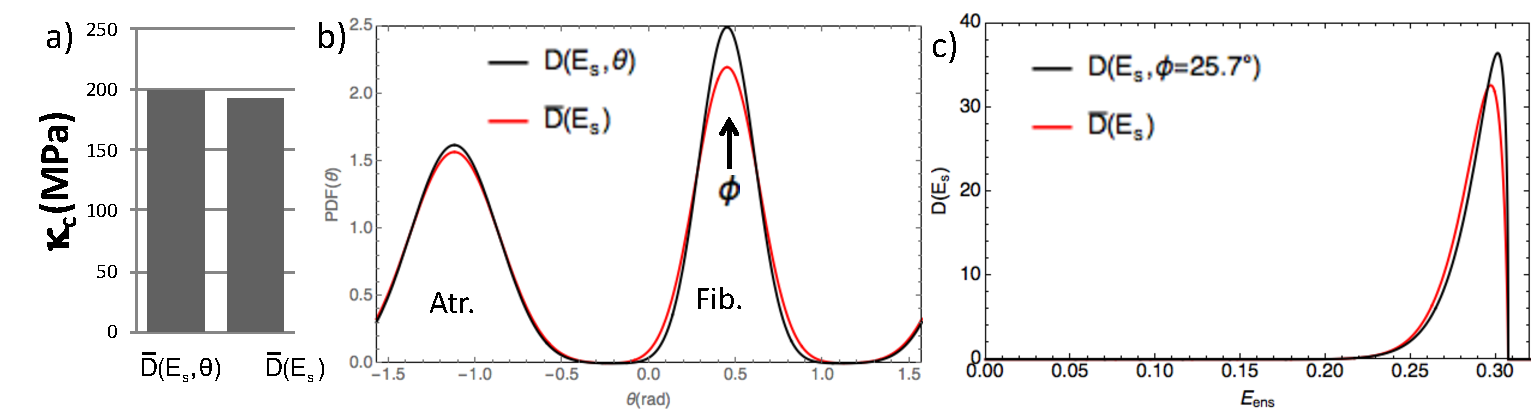
\includegraphics[width=\textwidth]{Images/chapter2/figure6.pdf}
\caption{The specimen was fit using both the comparisons for the orientation-variant $\bar{D}(\bar{\mathbf{\xi}},x)$ (Black) and orientation invariant $D(\mathbf{\xi},x,\mathbf{n}_0)$ (Red) modeling approaches for the recruitment functions. Both methods produce (a) nearly the same collagen fiber modulus. (b) The fiber ODFs also appears to the equivalent width ($\sigma_c^f$). (c) The recruitment distribution also appears to be similar.}
\label{c2:fig:6}
\end{figure}
%%%%%%%%%%%%%%%%%%%%	 end FIGURE 	%%%%%%%%%%%%%%%%%%%%
    
    
    The optimal recruitment parameters for both the multi-protocol data and the EB strain data were very similar (Table \ref{c2:tab:5}, \ref{c2:tab:6}, \ref{c2:tab:7}). We found no significant differences in the averaged standard deviation of recruitment, $\sigma_r$, between the anterior and posterior leaflets for either tests (Fig. \ref{c2:fig:5}b). There were minor differences in the distributions due to the way the upper-bound parameter was determined. The analysis of the EB strain kinematic state was done visually, where the upper-bound may have been underestimated. For analysis of the stress controlled planar biaxial tests, which does not reach full recruitment, the upper-bound was predicted by the parameter estimation algorithm and tended to be slightly overestimated. Uniaxial testing instead shows a very different recruitment response (Table \ref{c2:tab:4}). This is most likely due to the vastly different testing modes, where the differences in preconditioning and gauge length result in a drastically different reference state for the fibers. Additionally, fiber rotation effects in the uniaxial testing slow the recruitment of fibers away from the test axis and produce a greater standard deviation for the recruitment distribution. We however observe in trend that the posterior leaflet recruits slower than the anterior leaflet (Fig. \ref{c2:fig:5}b), possibly due to differences in their role mechanically during valve closure.
    
    


\subsection{Parameter validation} \label{c2:sec:233}

    Perhaps the most important validation finding was that the simulated SAXS response (Eqn. \ref{c2:eqn:fibrilstrain}), using the best fit parameters, matched very well to the MV SAXS data from Liao et al. \cite{liao_relation_2007} (Fig. \ref{c2:fig:7}). The squared correlation coefficient was computed ($r^2 = 0.971$), and we found no statistical significance ($p = 0.285$) between the two curves. To assess the sensitivity of the SAXS simulation (Eqn. \ref{c2:eqn:fibrilstrain}), the origin recruitment distribution parameters $\mu_r^f = 0.286$ and $E_{ub}^f = 0.307 $ were shifted by $\pm0.01$ in Green Lagrange strain, and the standard deviation of the collagen fiber ODF $\sigma_r^f = 10.3^\circ (\Gamma_c(\theta))$ was adjusted by $\pm1^\circ$ (Fig. \ref{c2:fig:7}). Despite the perturbation being so small, there was a 54\% increase in the slope of the simulated SAXS response when the mean and upper-bound of the recruitment was increased by 0.01, and a 38\% decrease in slope when the parameters were decreased by 0.01. Similarly, the slope decreased by 17\% when  was increased by $1^\circ$, and increased by 20\% when decreased by $1^\circ$. 
    An estimate of the fiber modulus for the MV SAXS data was made by comparing against the simulated data. No statistical significance for the collagen fiber modulus between any mechanical tests or between either leaflets was found. In addition, the predicted ODFs $\Gamma_c(\theta)$ and $\Gamma_e(\theta)$ compared very well with the SHG measurements, with standard deviations differing by no more than 3 degrees (Fig. \ref{c2:fig:8}). Thus, despite the model complexity, these validation results suggest that the parameters were sufficiently independent and each can be accurately determined as a representation of the mechanical behavior of the MV.
    
    
%%%%%%%%%%%%%%%%%%%%	begin FIGURE 	%%%%%%%%%%%%%%%%%%%%
\begin{figure}
\centering
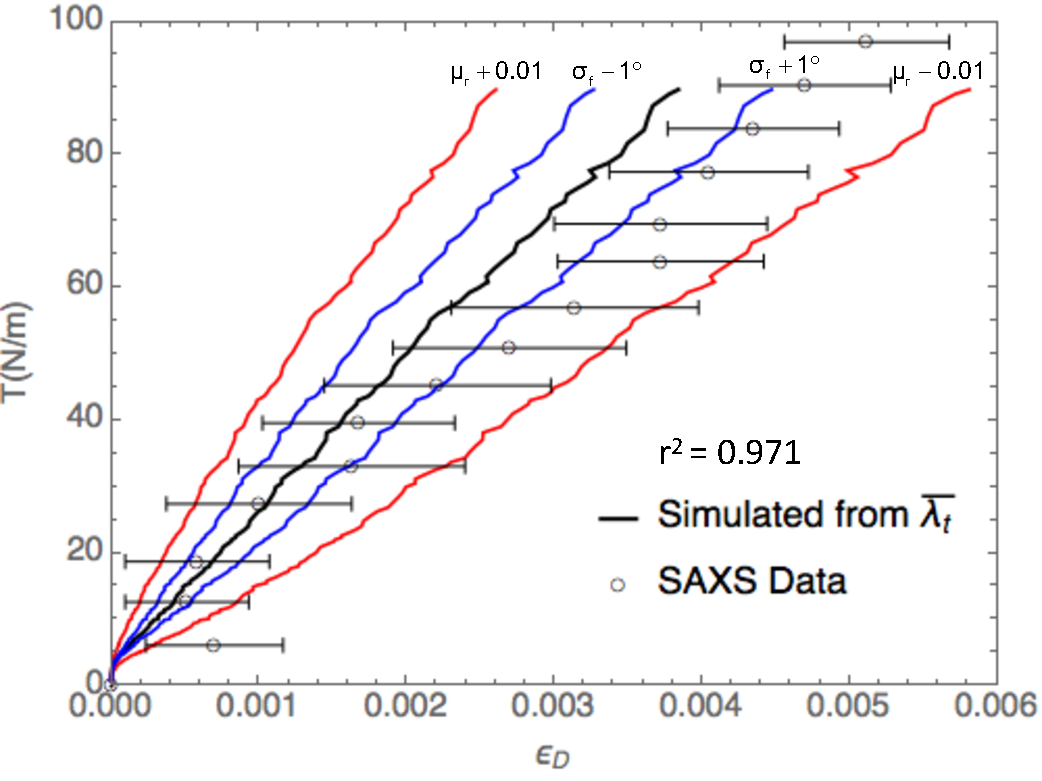
\includegraphics[width=0.75\textwidth]{Images/chapter2/figure7.pdf}
\caption{Collagen fibril stress–strain data from SAXS studies from Liao et al. \cite{liao_relation_2007} (circles) along with the simulated result based on the current model parameters (Black) showing very good agreement. This approach is very sensitive. Perturbing the ODF ($\sigma_c^f$) by $1^\circ$ (Blue) and shifting the recruitment distribution by 0.01 in Green strain (Red) significantly changed the slop of the curve.}
\label{c2:fig:7}
\end{figure}
%%%%%%%%%%%%%%%%%%%%	 end FIGURE 	%%%%%%%%%%%%%%%%%%%%


%%%%%%%%%%%%%%%%%%%%	begin FIGURE 	%%%%%%%%%%%%%%%%%%%%
\begin{figure}
\centering
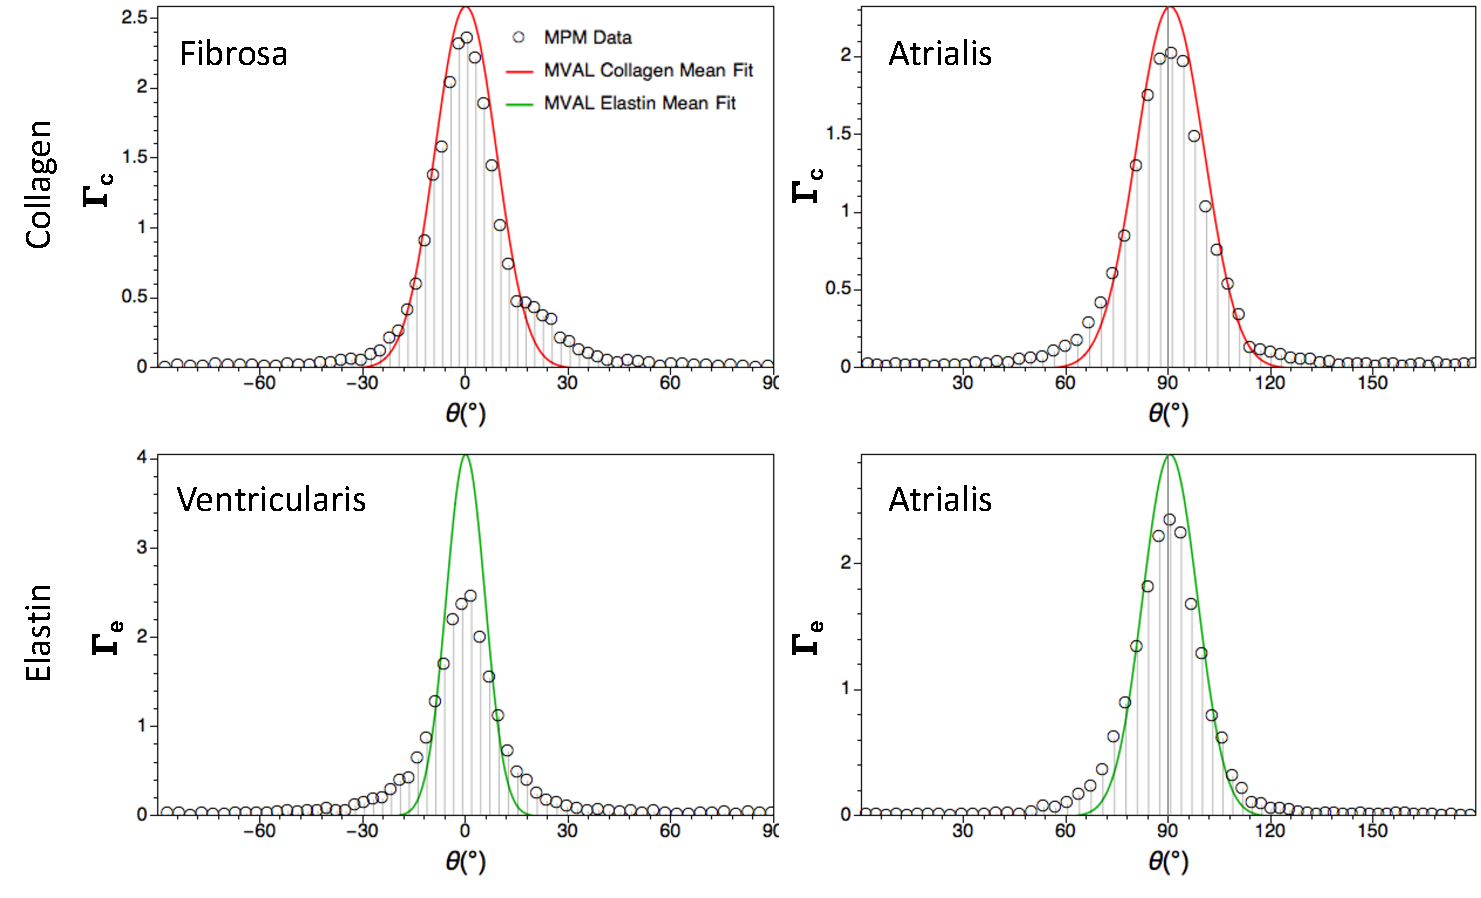
\includegraphics[width=\textwidth]{Images/chapter2/figure8.pdf}
\caption{The fitted orientation distribution functions of the collagen (Red) and elastin (Green) for the anterior leaflet are shown in comparison to the measured distribution from SHG (circle). The results are shown for the ventricularis, fibrosa and atrialis. The fitted and measured ODF appears to show good agreement. }
\label{c2:fig:8}
\end{figure}
%%%%%%%%%%%%%%%%%%%%	 end FIGURE 	%%%%%%%%%%%%%%%%%%%%




\subsection{Differences between layers and leaflets}

    All ODFs $\Gamma(\theta)$ of the ventricularis, fibrosa and atrialis were much narrower in the anterior leaflets than the posterior leaflets (Fig. \ref{c2:fig:9}). To estimate the mean ensemble elastin response, each elastin ensemble was scaled by the principle strain at maximum loading under EB stress and then averaged. Like the structural differences between the anterior and posterior leaflets, the mechanical response of ventricularis was much stiffer in the anterior leaflets comparing to the posterior leaflet (Fig. \ref{c2:fig:10}). On the other hand, the atrialis was stiffer in the posterior leaflet (Fig. \ref{c2:fig:10}). For the overall layer contributions, the mechanical response of the circumferential direction is mainly due to the elastin in the ventricularis at lower stress and the collagen within the fibrosa at high stress, whereas the radial direction is a combination of collagen fibers in the fibrosa as they extend and rotate under physiological loading and collagen in the atrialis at higher strains (Fig. \ref{c2:fig:11}). The mechanical contribution from the spongiosa was, as anticipated, negligible for both leaflets.
    
    
%%%%%%%%%%%%%%%%%%%%	begin FIGURE 	%%%%%%%%%%%%%%%%%%%%
\begin{figure}
\centering
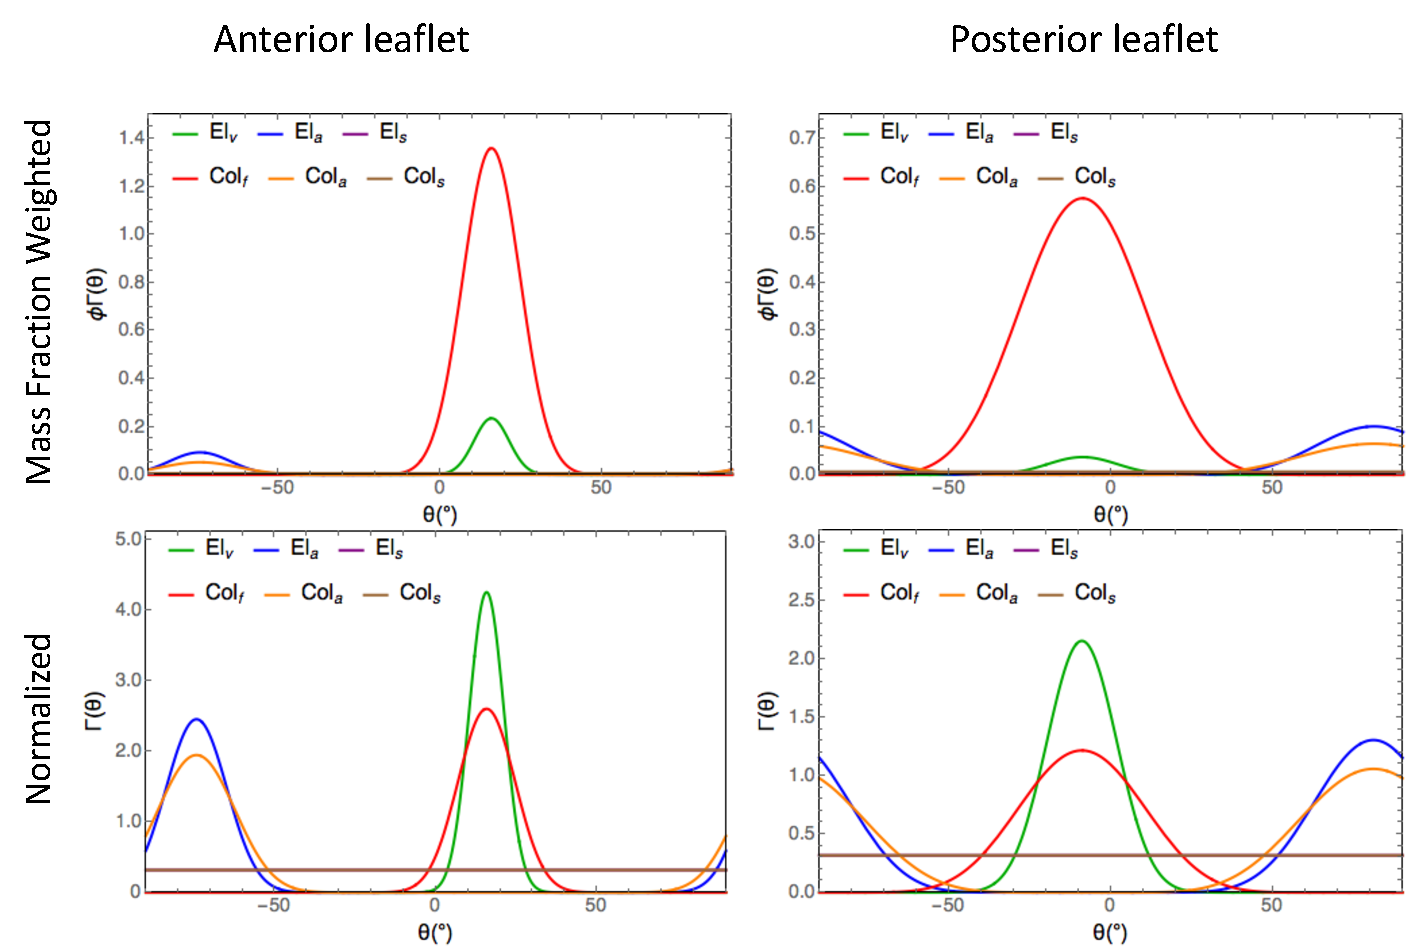
\includegraphics[width=\textwidth]{Images/chapter2/figure9.pdf}
\caption{The predicted fiber orientation distributions from the anterior (Left) and posterior leaflets (Right) for collagen and elastin from all layers as an average (n = 7 for both leaflets). Both the mass fraction scaled (Top) and normalized (Both) ODFs are shown. In both leaflets the collagen of the fibrosa layer is clearly the most dominant, but is more broadly distributed in the posterior leaflet. Elastin is also similarly trends but is more evenly distributed in the anterior leaflet, while favoring the atrialis in the posterior leaflet.}
\label{c2:fig:9}
\end{figure}
%%%%%%%%%%%%%%%%%%%%	 end FIGURE 	%%%%%%%%%%%%%%%%%%%%


%%%%%%%%%%%%%%%%%%%%	begin FIGURE 	%%%%%%%%%%%%%%%%%%%%
\begin{figure}
\centering
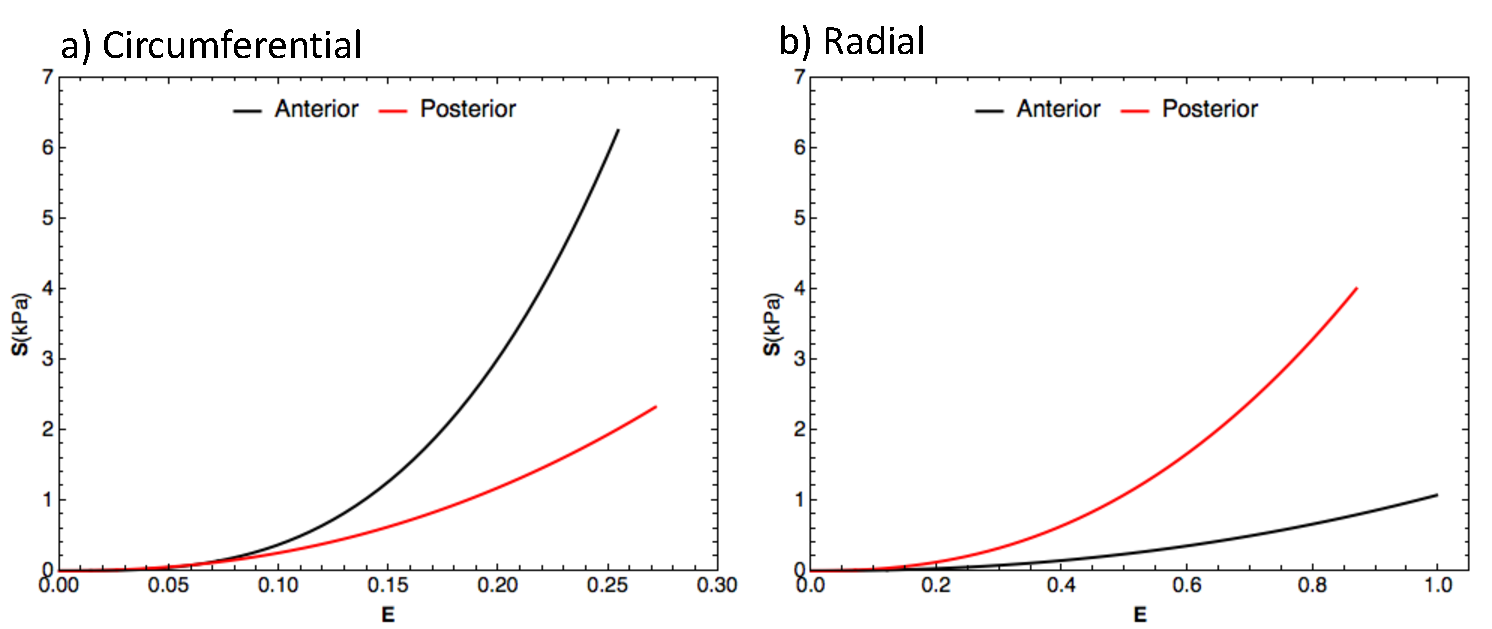
\includegraphics[width=\textwidth]{Images/chapter2/figure10.pdf}
\caption{The mean elastin response in the physiological range from both anterior (Black) and posterior (Red) leaflets in the circumferential (a) and radial (b) directions. n = 7 for both leaflets. The elastin in the anterior leaflet is heavily anisotropy and favoring the circumferential direction, which the elastin in the posterior leaflet is more isotropic and only slightly favoring the radial direction.}
\label{c2:fig:10}
\end{figure}
%%%%%%%%%%%%%%%%%%%%	 end FIGURE 	%%%%%%%%%%%%%%%%%%%%


%%%%%%%%%%%%%%%%%%%%	begin FIGURE 	%%%%%%%%%%%%%%%%%%%%
\begin{figure}
\centering
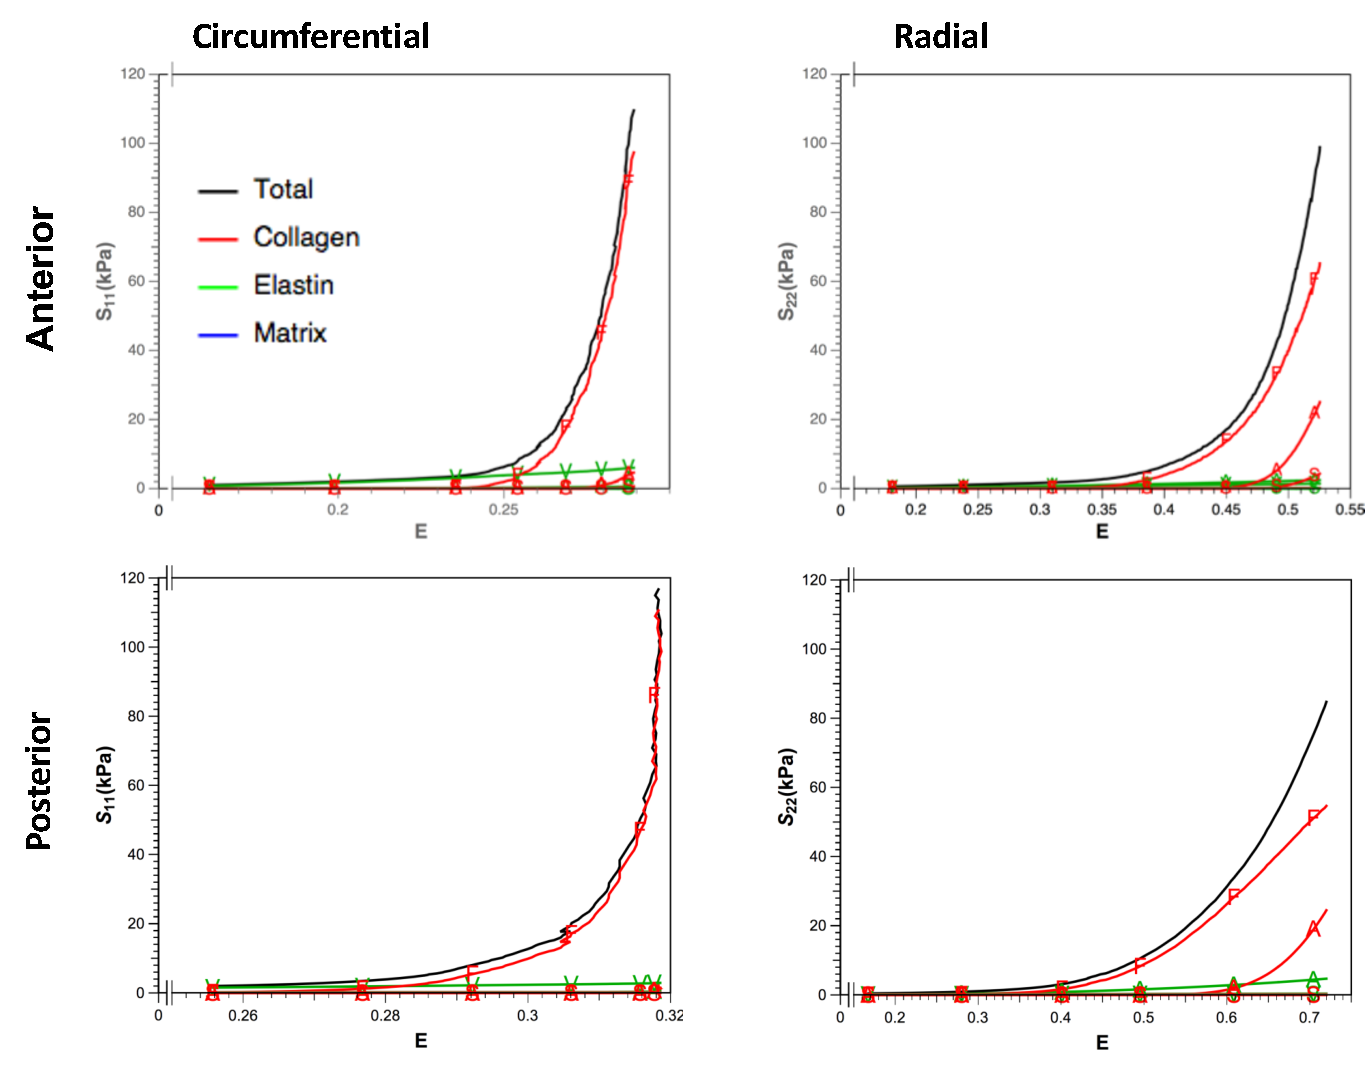
\includegraphics[width=\textwidth]{Images/chapter2/figure11.pdf}
\caption{The net stress contribution from each ECM component from each layer for the equibiaxial stress protocol is shown for the circumferential (Left) and radial (Right) direction of the anterior (Top) and posterior (Bottom) leaflets. Here, the contributions from the layers are ventricularis (V), fibrosa (F), spongiosa (S), and atrialis (A). Interestingly, while the fibrosa layer is dominant circumferential directions in both leaflets, the atrialis also contributes substantially in the radial direction. Elastin clearly contributes minimal stress comparing to collagen, but it forms the bulk of the response in the toe region.}
\label{c2:fig:11}
\end{figure}
%%%%%%%%%%%%%%%%%%%%	 end FIGURE 	%%%%%%%%%%%%%%%%%%%%




